% 0064(본책 16쪽) — ∠B=90° 직각삼각형 ABC(A 위·B 왼쪽 아래·C 오른쪽 아래), D 는 BC 위, E 는 AC 위, DE⊥AC. 라벨: A·B·C·D·E, 7(DE)·9(DC) 파선 호, 각 x(∠A), 직각 표시 B·E. 스캔 삽화를 TikZ 로 다시 그림. 답(sin x/tan x)은 적지 않는다.
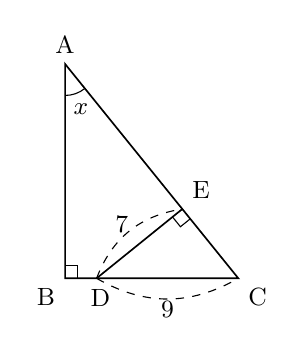
\begin{tikzpicture}[scale=1, line width=0.6pt]
  \coordinate (B) at (0,0); \coordinate (C) at (2.2,0); \coordinate (A) at (0,2.722); \coordinate (D) at (0.4,0); \coordinate (E) at (1.489,0.8797);
  \draw (A) -- (B) -- (C) -- cycle;
  \draw (D) -- (E);
  % 직각 표시
  \draw[line width=0.4pt] (0.16,0) -- (0.16,0.16) -- (0,0.16);
  \draw[line width=0.4pt] (1.3645,0.7792) -- (1.4651,0.6548) -- (1.5896,0.7553);
  % 각 x(∠A)
  \draw[line width=0.4pt] (0,2.322) arc[start angle=-90, end angle=-51.06, radius=0.4cm];
  \node[font=\small] at (0.2,2.15) {$x$};
  % 길이(파선 호)
  \draw[dashed, line width=0.4pt] (D) to[bend left=30] (E);
  \draw[dashed, line width=0.4pt] (D) to[bend right=30] (C);
  \node[font=\small] at (0.72,0.68) {$7$};
  \node[font=\small] at (1.3,-0.4) {$9$};
  \node[font=\small, above] at (A) {A};
  \node[font=\small, below left] at (B) {B};
  \node[font=\small, below right] at (C) {C};
  \node[font=\small, below] at (0.45,-0.02) {D};
  \node[font=\small, above right] at (E) {E};
\end{tikzpicture}
